% 08
\begin{frame}[t]{Android 6: Ai làm phần xác minh?}
  \noindent
  \begin{minipage}[t]{.32\linewidth}\vspace{0pt}
    \SemBlueCard{Hồ sơ AOSP}{%
      \SemCode{1c1b471}\par\smallskip
      \textbf{Add IntentFilter auto verification}\par\smallskip
      Fabrice Di Meglio\par
      \small Đóng góp triển khai}
  \end{minipage}\hfill
  \begin{minipage}[t]{.64\linewidth}\vspace{0pt}
    \begin{tabularx}{\linewidth}{@{}L{.34\linewidth}Y@{}}
      \toprule
      \textbf{Mốc} & \textbf{Dấu vết lịch sử}\\
      \midrule
      19/11/2014\newline
      \(\rightarrow\) 30/03/2015 &
        Ngày tác giả và ngày commit trong AOSP.\\[.22em]
      28/05/2015 &
        Jamal Eason giới thiệu App Links trong Android M Preview.\\[.22em]
      10/2015 &
        Android 6.0 (API 23) phát hành App Links.\\
      \bottomrule
    \end{tabularx}
  \end{minipage}\par\smallskip

  \SemCallout{Mục tiêu trong AOSP là giảm số lần Android hỏi người dùng chọn app.}
  \SemSource{\href{https://android.googlesource.com/platform/frameworks/base/+/1c1b47125da018b44240739db75f8898e064a948}{Commit AOSP}
    · \href{https://android-developers.googleblog.com/2015/05/android-m-developer-preview-tools.html}{Android M Preview}
    · \href{https://developer.android.com/about/versions/marshmallow/android-6.0\#app-linking}{Android 6.0 APIs}}
\end{frame}

% 09
\begin{frame}[t]{Xác minh khi thiết lập, phân giải khi bấm}
  \noindent\makebox[\linewidth][c]{%
    \begin{tikzpicture}[x=1mm,y=1mm,
      sem diagram box/.style={draw=Rule,fill=Paper,text=Ink,text width=31mm,align=center,
        minimum height=12mm,inner sep=1.6mm,font=\small},
      sem core box/.style={sem diagram box,fill=Navy,draw=Navy,text=white},
      sem next arrow/.style={-{Stealth[length=1.75mm]},Action,line width=.65pt}]
      \node[anchor=west,inner sep=0pt] at (2,51) {\SemLabel{01 · THIẾT LẬP QUAN HỆ}};
      \node[sem diagram box] (apk) at (19,40) {\textbf{APK}\\Phạm vi URL + \SemCode{autoVerify}};
      \node[sem core box] (verify) at (67,40) {\textbf{Android xác minh}\\So ID và SHA-256};
      \node[sem diagram box] (website) at (115,40) {\textbf{Website}\\Tuyên bố qua HTTPS};
      \draw[sem next arrow] (apk.east) -- (verify.west);
      \draw[sem next arrow] (website.west) -- (verify.east);

      \node[anchor=west,inner sep=0pt] at (2,23) {\SemLabel{02 · KHI CÓ LẦN BẤM}};
      \node[sem diagram box] (tap) at (19,12) {\textbf{Cú bấm}\\Web Intent};
      \node[sem core box] (resolve) at (67,12) {\textbf{Android phân giải}\\Bộ lọc và cài đặt};
      \node[sem diagram box] (dest) at (115,12) {\textbf{Nơi nhận URL}\\App hoặc trình duyệt};
      \draw[sem next arrow] (tap.east) -- (resolve.west);
      \draw[sem next arrow] (resolve.east) -- (dest.west);
      \draw[sem next arrow,dashed] (verify.south) --
        node[right,fill=white,text=Slate,inner sep=1.2mm,font=\footnotesize]{Trạng thái đã ghi} (resolve.north);
    \end{tikzpicture}%
  }\par
  \noindent\SemLabel{Manifest}\quad\SemCode{android:autoVerify="true"}\par
  \noindent\SemLabel{Đúng host HTTPS}\quad\SemCode{/.well-known/assetlinks.json}\par
  \SemSource{\href{https://developer.android.com/training/app-links/about}{About App Links}
    · \href{https://developer.android.com/training/app-links/verify-applinks}{Verify App Links}}
\end{frame}

% 10
\begin{frame}[t]{Tại sao cần cả ID và dấu vân tay?}
  \SemCallout{\textbf{Website ủy quyền}\quad ID \textbf{P} · dấu vân tay chứng chỉ \textbf{B}}
  \medskip
  \noindent\SemLabel{BA TÌNH HUỐNG CÀI ĐẶT ĐỘC LẬP}\par\smallskip
  {%
    \setlength{\tabcolsep}{4pt}
    \begin{tabularx}{\linewidth}{L{.28\linewidth}L{.18\linewidth}L{.155\linewidth}Y}
      \toprule
      \textbf{Bản đang cài} & \textbf{ID ứng dụng} & \textbf{SHA-256} & \textbf{So với tuyên bố}\\
      \midrule
      Bản thử nghiệm & P & A & Chỉ khớp ID.\\
      \rowcolor{Ice} Bản phát hành & \textbf{P} & \textbf{B} & \textcolor{Action}{\textbf{Khớp cả hai.}}\\
      App khác, cùng bên ký & Q & B & Chỉ khớp dấu vân tay.\\
      \bottomrule
    \end{tabularx}\par
  }
  \medskip
  \noindent\SemLabel{KHI CÀI APK}\enspace Android kiểm chữ ký bằng khóa công khai trong chứng chỉ.\par\smallskip
  \noindent\SemLabel{KHI XÁC MINH HOST}\enspace Android so ID và SHA-256 của chứng chỉ đó.\par
  \SemSource{\href{https://developers.google.com/digital-asset-links/reference/rpc/google.digitalassetlinks.v1\#androidappasset}{Định danh Digital Asset Links}
    · \href{https://source.android.com/docs/security/features/apksigning/v2\#verification}{Kiểm tra chữ ký APK}}
\end{frame}

% 11
\begin{frame}[t]{Android 12 quy định đường về trình duyệt}
  \SemLabel{2021 · API 31 · YÊU CẦU MỞ LINK WEB THÔNG THƯỜNG}\par\medskip

  \noindent\makebox[\linewidth][c]{%
    \begin{tikzpicture}[x=1mm,y=1mm,
      sem diagram box/.style={draw=Rule,fill=Paper,text=Ink,text width=26mm,align=center,inner sep=1.7mm,minimum height=9mm},
      sem next arrow/.style={-{Stealth[length=1.75mm]},Action,line width=.65pt}]
      \node[sem diagram box] (web) at (15,18) {Web Intent};
      \node[sem diagram box,draw=Navy,fill=Navy,text=white,text width=33mm] (resolve) at (63,18)
        {App khớp URL và được chấp thuận?};
      \node[sem diagram box] (app) at (117,26) {Activity của app};
      \node[sem diagram box] (browser) at (117,10) {Trình duyệt mặc định};
      \draw[sem next arrow] (web.east) -- (resolve.west);
      \draw[sem next arrow] (resolve.east) -- (91,18) |-
        node[pos=.78,above,text=Action,font=\footnotesize]{Có} (app.west);
      \draw[sem next arrow] (91,18) |-
        node[pos=.63,below,text=Slate,font=\footnotesize]{Không} (browser.west);
      \node[anchor=north,text=Slate,font=\footnotesize] at (browser.south) {Cùng URL};
    \end{tikzpicture}%
  }\par\smallskip

  \SemCallout{Chấp thuận cho tên miền có thể đến từ xác minh App Links hoặc lựa chọn trong cài đặt Android.}
  \SemSource{\href{https://developer.android.com/about/versions/12/behavior-changes-all\#web-intent-resolution}{Android 12: phân giải web Intent}}
\end{frame}

% 12
\begin{frame}[t]{Công tắc làm đổi nơi mở}
  \noindent\makebox[\linewidth][c]{%
    \begin{tikzpicture}[x=1mm,y=1mm,
      sem leader/.style={Action,line width=.6pt}]
      \node[anchor=south west,inner sep=0pt] at (5,2)
        {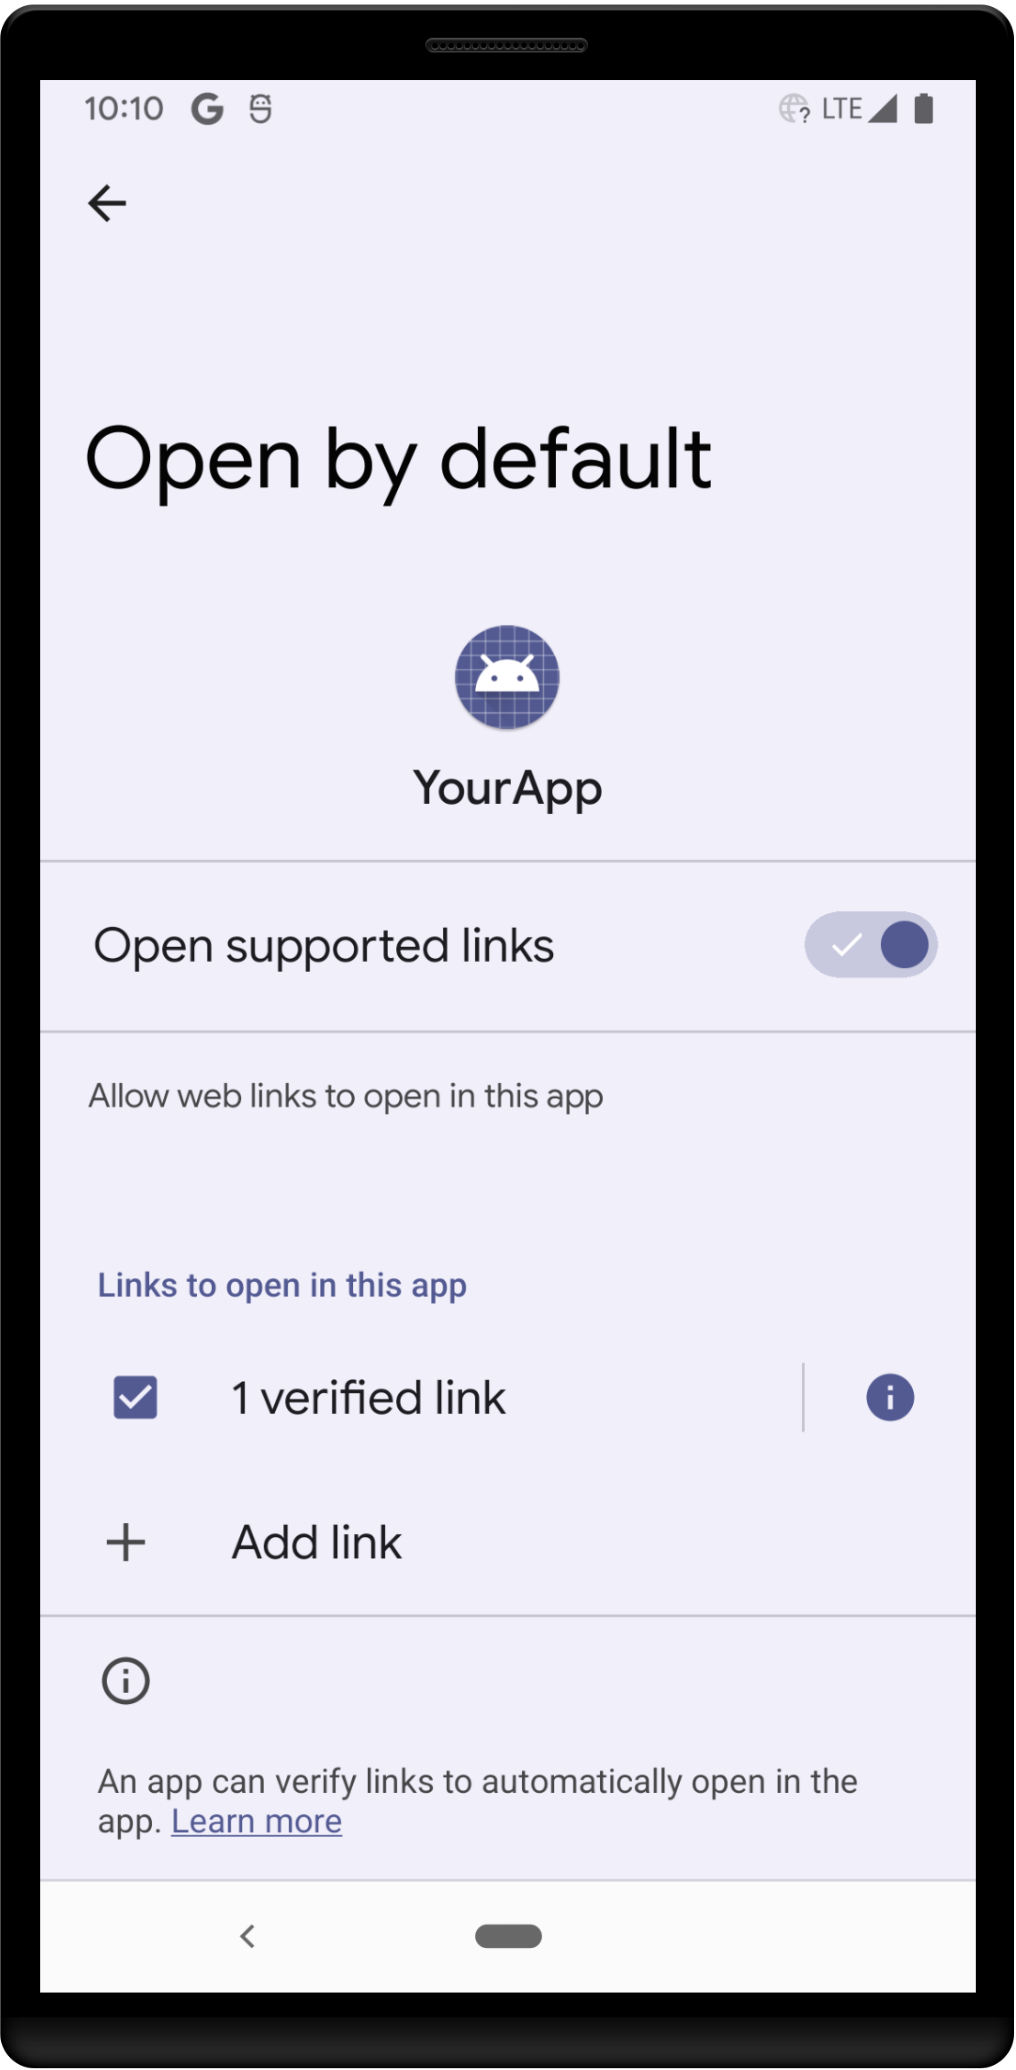
\includegraphics[height=46mm]{assets/platform/choose-domains.png}};
      \draw[sem leader] (26.1,27.4) -- (33,27.4) -- (39,36.5) -- (43,36.5);
      \draw[sem leader] (26.1,17.1) -- (33,17.1) -- (39,19.5) -- (43,19.5);
      \fill[Action] (26.1,27.4) circle (.7mm);
      \fill[Action] (26.1,17.1) circle (.7mm);
      \node[anchor=west,inner sep=0pt,text width=88mm] at (45,36.5) {%
        \SemLabel{QUYỀN MỞ LINK}\par
        \textbf{Open supported links}\enspace Người dùng có cho app mở link không?};
      \node[anchor=west,inner sep=0pt,text width=88mm] at (45,19.5) {%
        \SemLabel{XÁC MINH TÊN MIỀN}\par
        \textbf{1 verified link}\enspace Android đã ghi nhận quan hệ với website chưa?};
      \node[anchor=south west,inner sep=0pt,text=Slate,text width=88mm,font=\small] at (45,1.2) {%
        Khi tắt công tắc, URL có thể về trình duyệt dù quan hệ tên miền vẫn được xác minh.};
    \end{tikzpicture}%
  }\par
  \SemSource{\href{https://developer.android.com/training/app-links/verify-applinks\#make-the-request}{Android Developers · Màn hình của app mẫu YourApp}}
\end{frame}

% 13
\begin{frame}[t]{Dynamic App Links và phạm vi APK}
  \SemLead{Ví dụ web: giữ lịch cũ trên trình duyệt trong phạm vi \SemCode{/schedule/}.}

  \noindent
  \begin{minipage}[t]{.36\linewidth}\vspace{0pt}
    \begin{tikzpicture}[x=1mm,y=1mm,
      sem marker/.style={circle,draw=Navy,fill=white,text=Ink,inner sep=0pt,minimum size=4.5mm,font=\footnotesize\bfseries}]
      \path[fill=Ice,draw=Rule,line width=.5pt] (0,0) rectangle (44,31);
      \node[anchor=north west,inner sep=0pt] at (2.7,28.5) {\SemLabel{Phạm vi manifest}};
      \path[fill=Navy] (2.7,4) rectangle (31,21);
      \node[anchor=west,text=white,text width=26mm,inner sep=0pt,font=\footnotesize\bfseries]
        at (4.4,17.2) {URL mở app};
      \node[sem marker] at (16,10) {1};
      \node[sem marker] at (37.2,10) {2};
      \node[sem marker] at (48.5,10) {3};
    \end{tikzpicture}
  \end{minipage}\hfill
  \begin{minipage}[t]{.61\linewidth}\vspace{0pt}
    \begin{tabularx}{\linewidth}{@{}L{.51\linewidth}Y@{}}
      \toprule
      \textbf{Đường dẫn minh họa} & \textbf{Hành vi}\\
      \midrule
      1 · {\footnotesize\SemCode{/schedule/2026-11-25}} & Có thể mở app.\\[.18em]
      2 · {\footnotesize\SemCode{/schedule/archive/2024}} & Quy tắc động loại, về web.\\[.18em]
      3 · {\footnotesize\SemCode{/news/today}} & Ngoài phạm vi APK, không thể thêm.\\
      \bottomrule
    \end{tabularx}
  \end{minipage}\par\smallskip

  \SemCallout{Khả dụng từ năm 2025 trên Android 15+ có Google services. Thiết bị cập nhật quy tắc theo chu kỳ.}
  \SemSource{\href{https://developer.android.com/training/app-links/configure-assetlinks\#order-dynamic-rules}{Quy tắc động và thứ tự khớp}
    · \href{https://developer.android.com/blog/posts/dynamic-app-links-elevating-your-android-deep-linking}{Thông báo của Ran Mor}}
\end{frame}
